Gli esseri umani, talvolta senza rendersene conto, riescono a integrare continuamente nuove informazioni riguardo l'ambiente che li circonda, sia esso una casa, un edificio pubblico o un parco. Questa capacità, conscia e inconscia, è essenziale per la successiva pianificazione di quei obiettivi o movimenti basati sulle informazioni appena apprese. \\
Così come per gli essere umani, anche i robot hanno bisogno di informazioni per poter essere considerati "cognitivi" e pianificare rispetto alla propria base di conoscenza. In particolar modo quando l'obiettivo è pianificare missioni data la descrizione in linguaggio in naturale di ciò che il robot deve fare, come in questo caso.

\paragraph*{Esempio}
Consideriamo una persona che entra per la prima volta in una biblioteca. Egli osserva scaffali pieni di libri, tavoli per lo studio e un'area dedicata ai computer. Queste informazioni vengono immagazzinate e utilizzate successivamente per trovare un libro specifico o un luogo tranquillo per studiare.\\
Allo stesso modo, immaginiamo un robot progettato per operare in una casa intelligente. Riceve l'istruzione: "Prendi il libro dal tavolo del soggiorno e portalo in cucina." Per svolgere questo compito, il robot deve comprendere la struttura della casa, identificare il tavolo corretto e navigare verso la cucina.

\section{Definizione}
La Mappa Semantica è un grafo orientato $G_m = (V_m, E_m)$ che rappresenta questa base di conoscenza dove:
% Riscrivere le liste dal punto di vista dei nodi
\begin{itemize}
  \item Un nodo può essere un:
        \begin{itemize}
          \item Nodo stanza;
          \item Nodo oggetto;
          \item Nodo tag.
        \end{itemize}
  \item Un arco può rappresentare:
        \begin{itemize}
          \item La relazione tra due oggetti;
          \item Il collegamento tra due stanze;
          \item L'appartenenza di un oggetto o un tag ad una ed una sola stanza.
        \end{itemize}
\end{itemize}
Di conseguenza, per trovare gli oggetti o i nodi appartenenti ad una stanza $s$ è sufficiente considerare il sottografo del nodo stanza $s$.

\begin{figure}[h]
  \begin{subfigure}[t]{0.45\textwidth}
    \centering
    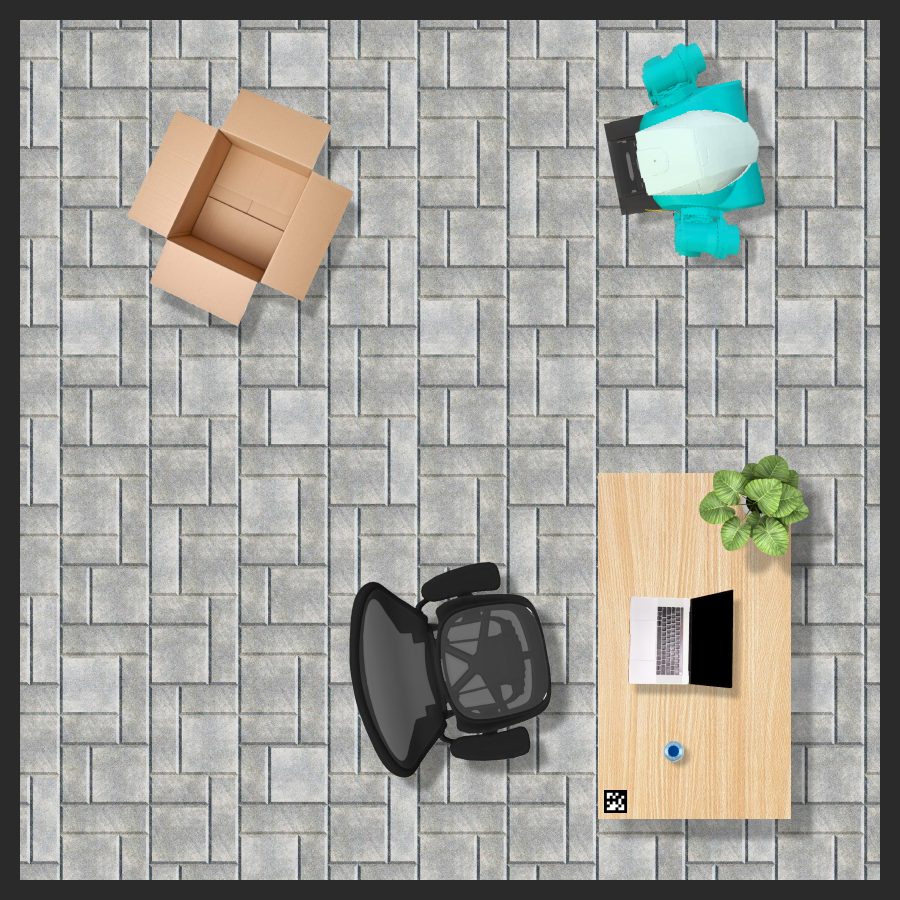
\includegraphics[width=0.98\textwidth]{commons/scene_all.png}
    \caption{Ambiente circostante il robot \textit{(posizionato in alto a destra)}}
  \end{subfigure}
  \begin{subfigure}[t]{0.55\textwidth}
    \centering
    \begin{tikzpicture}[
      >={Stealth[round]},  % Arrow tip
      auto,
      thick  % Line thickness
      ]
      \node (a) [circle, draw, scale=0.8, fill=green!20] {Ufficio};

      \begin{scope}[node distance=1.2cm and 0.62cm]
        \node (g) [circle, draw, scale=0.7, above=of a] {Box};
        \node (h) [circle, draw, scale=0.7, right=of g, fill=blue!20] {Tag};
        \node (i) [circle, draw, scale=0.7, left=of g] {Floor};
      \end{scope}

      \begin{scope}[node distance=1.2cm and 0.62cm]
        \node (d) [circle, draw, scale=0.7, below=of a] {Table};
        \node (b) [circle, draw, scale=0.7, left=of d] {Laptop};
        \node (c) [circle, draw, scale=0.7, left=of b] {Plant};
        \node (e) [circle, draw, scale=0.7, right=of d] {Chair};
        \node (f) [circle, draw, scale=0.7, right=of e] {Bottle};
      \end{scope}

      \foreach \node in {b,c,d,e,f,g,h,i}
      \draw[<->] (a) -- (\node);

      \draw[->] (c) to [bend right=40] node[midway, below] {\tiny{on}} (d);
      \draw[->] (f) to [bend left=40] node[midway, below] {\tiny{on}} (d);
      \draw[->] (b) to [bend right=20] node[midway, below] {\tiny{on}} (d);
      \draw[->] (c) to [bend right=20] node[midway, below] {\tiny{near}} (b);
      \draw[->] (e) to [bend left=20] node[midway, below] {\tiny{near}} (d);
      \draw[->] (d) to [bend left=20] node[midway, above] {\tiny{near}} (e);
      \draw[->] (g) to [bend right=20] node[midway, above] {\tiny{on}} (i);
    \end{tikzpicture}
    \caption{In verde in nodi stanza, in blu i nodi tag e in bianco i nodi oggetto.}
  \end{subfigure}
  \caption{Ambiente e relativa mappa semantica. }
\end{figure}

\subsection{Nodi}
\subsubsection{Nodi oggetto}

I nodi oggetto rappresentano gli oggetti riconosciuti all'interno dell'ambiente attraverso la segmentazione panoptica dei frame video proveniente dalle camere del robot. Ogni nodo oggetto ha i seguenti attributi:
\begin{itemize}
  \item Identificativo: utilizzato per identificare un oggetto all'interno della Mappa Semantica;
  \item Nome: label inferita dal modello di segmentazione panoptica;
  \item Posizione: terna $(x, y, z)$ rappresentante la posizione dell'oggetto all'interno dell'ambiente rispetto alla Reference Posizione;
  \item Reference Posizione: origine del sistema di riferimento delle posizioni degli oggetti. Può essere l'origine del sistema Mappa o l'origine del sistema Robot;
  \item Tipo: rappresenta la tipologia dell'oggetto che può essere scelta tra:
        \begin{itemize}
          \item Living Entity: entità vivente;
          \item Unpickable Object: qualora l'oggetto non possa essere preso attraverso gli end effectors del robot;
          \item Pickable Object: qualora l'oggetto possa essere preso attraverso gli end effectors del robot;
          \item Placeable Asset: qualora l'oggetto possa essere spostato ma non preso;
          \item Unplaceable Asset: qualora l'oggetto non possa essere spostato.
        \end{itemize}
\end{itemize}
I nodi oggetto vengono aggiornati con le inferenze di nuovi frame video: possono dunque essere eliminati dalla mappa semantica qualora un oggetto non si presenti più all'interno della scena oppure aggiornati, per esempio a livello di posizione, qualora l'oggetto venga spostato.

\begin{figure}[h]
  \centering
  \begin{tikzpicture}
    \subfile{uml/basic_node}
    \subfile{uml/object_node}

    \umlinherit[ geometry=-- ]{BasicNode}{ObjectNode}
  \end{tikzpicture}
  \caption{Diagramma delle classi - Nodo Oggetto}
\end{figure}

\subsubsection{Nodi tag}
I nodi tag rappresentano tutti quei riferimenti che vengono utilizzati dal robot per localizzarsi o localizzare oggetti di particolare rilevanza (come la stazione di ricarica o il tavolo di lavoro). Ogni nodo tag ha i seguenti attributi:
\begin{itemize}
  \item Identificativo: utilizzato per identificare il tag all'interno della Mappa Semantica;
  \item Nome: assegnato dall'utente;
  \item Posizione: terna $(x, y, z)$ rappresentante la posizione del tag all'interno dell'ambiente rispetto all'origine della mappa;
  \item Dimensione: dimensione del tag in millimetri;
  \item Di Navigazione: flag che indica se il tag è utilizzato per la navigazione del robot;
  \item Per Picking: flag che indica se il tag è utilizzato per identificare un oggetto di cui fare il picking con gli end effectors.
\end{itemize}
I nodi tag sono permanenti all'interno della mappa semantica perché si assume che questi non vengano mai spostati o rimossi dall'ambiente del robot

\begin{figure}[h]
  \centering
  \begin{tikzpicture}
    \subfile{uml/basic_node}
    \subfile{uml/tag_node}

    \umlinherit{BasicNode}{ObjectNode}
  \end{tikzpicture}
  \caption{Diagramma delle classi - Nodo Tag}
\end{figure}

\subsubsection{Nodi stanza}
I nodi stanza rappresentano un'area semantica all'interno della mappa slam generata attraverso i sensori LiDaR del robot che, data in input ad un algormito, questo individua le stanze e ne genera il poligono.
Ogni nodo stanza ha i seguenti attributi:
\begin{itemize}
  \item Identificativo: utilizzato per identificare la stanza all'interno della Mappa Semantica;
  \item Nome: assegnato dall'utente;
  \item Segmenti: Lista di segmenti che delimitano il poligono della stanza. Viene usato per verificare se un oggetto appartiene ad una stanza o no;
  \item Oggetti: Sottografo degli oggetti appartenenti alla stanza.
\end{itemize}
La presenza di queste aree nella mappa è fondamentale per diverse ragioni:
\begin{itemize}
  \item Permette di suddividere gli oggetti rispetto alla stanza di appartenenza, facilitando la discriminazione degli omonimi in base alla stanza di appartenenza e aggiungendo \textbf{keypoint} per la descrizione in linguaggio naturale di una missione;
  \item Consentirà l'utilizzo di algoritmi di ricerca su grafo per la pianificazione del percorso per raggiungere gli oggetti;
  \item Permetterà di creare percorsi pianificati che evitano determinate stanze.
\end{itemize}

\begin{figure}[h]
  \centering
  \begin{tikzpicture}
    \umlclass[type=abstract, x=0, y=0]{BasicNode}{
  + id : String \\
  + name: String
}{

}
    \umlclass[x=5, y=0]{RoomNode}{
  + segments : List[List[Position]] \\
  + objects : ObjectsGraph
}{}

    \umlinherit{BasicNode}{RoomNode}
  \end{tikzpicture}
  \caption{Diagramma delle classi - Nodo Stanza}
\end{figure}
\subsection{Archi}
\subsubsection{Archi tra stanze}
Gli archi tra i nodi di tipo stanza rappresentano il collegamento diretto tra due stanze.
\subsubsection{Archi tra oggetti}
Gli archi orientati tra i nodi di tipo oggetto rappresentano la relazione tra due oggetti. L'etichetta associata ad ogni arco appartiene all'insieme delle relazioni che possono essere inferite dal modello PSGTr. Queste informazioni sono importanti per poter pianificare task all'interno della missione che supportano il raggiungimento dell'obiettivo.

Per esempio, immaginiamo la missione "Prendi la bottiglia". Se è presente un ostacolo davanti alla bottiglia, rispetto alla posizione di presa del robot, questo deve prima pianificare lo spostamento dell'ostacolo. Ecco il motivo per il quali vi è la necessità di rappresentare queste relazioni tra oggetti.

\subsection{Grafo stanze}
Definiamo il grafo delle stanze come il sottografo $(V_s, E_s)$ tale che:
\begin{itemize}
  \item $V_s = \{v \in V_m \mid v \text{ è un nodo stanza} \}$
  \item $E_s = \{(v,u) \in E_m \mid v \in V_s \wedge u \in V_s \}$
\end{itemize}
dove $V_m$ è l'insieme dei vertici del grafo della Mappa Semantica e $E_m$ è l'insieme degli archi del grafo della Mappa Semantica. \\\\
Questo grafo, viene generato a partire dall'algoritmo di riconoscimento delle stanze, illustrato nel Capitolo~\ref{chap:riconoscimento_stanze}, ed è la prima parte di Mappa Semantica creata, in concomitanza con la generazione della mappa slam. Solo successivamente sarà possibile la costruzione del grafo degli oggetti.
\subsection{Grafo Oggetti}
Definiamo il grafo degli oggetti (o grafo di scena) come il sottografo $(V_o, E_o)$ tale che:
\begin{itemize}
  \item $V_o = \{v \in V_m \mid v \text{ è un nodo oggetto o tag} \}$
  \item $E_o = \{(v,u) \in E_m \mid v \in V_o \wedge u \in V_o \}$
\end{itemize}
dove $V_m$ è l'insieme dei vertici del grafo della Mappa Semantica e $E_m$ è l'insieme degli archi del grafo della Mappa Semantica. \\\\
Una versione grezza del grafo degli oggetti viene generata dal modello PSGTr di \cite{yang2022psg}. Successivamente, come verrà mostrato nel Capitolo~\ref{chap:grafo_di_scena}, questa verrà fusa con la Mappa Semantica rendendo dunque la base di conoscenza coerente rispetto lo stato dell'ambiente attuale.

\subsection{Esempio di Mappa Semantica}
Di seguito un esempio di mappa semantica e i vari sottografi.

\begin{figure}[H]
  \begin{tikzpicture}[
    >={Stealth[round]},  % Arrow tip
    auto,
    node distance=2cm,  % Distance between nodes
    thick  % Line thickness
    ]
    \node (a) [circle, draw, fill=green!20] {Cucina};
    \node (b) [circle, draw, right =of a, fill=green!20 ] {Salotto};
    \node (c) [circle, draw, right =of b, fill=green!20] {Ingresso};

    \node (e) [circle, draw, below=of a] {Tavolo};
    \node (d) [circle, draw, left=of e] {Bottiglia};

    \node (f) [circle, draw, below =of b] {Persona};
    \node (g) [circle, draw, right =of f] {Laptop};

    \draw[<->] (a) -- (b);
    \draw[<->] (c) -- (b);

    \draw[->] (d) to [bend left=20] node[midway, above] {on} (e);
    \draw[->] (e) to [bend left=20] node[midway, below] {under} (d);
    \draw[<->] (a) -- (d);
    \draw[<->] (a) -- (e);

    \draw[->] (f) to [bend left=20] node[midway, above] {looking at} (g);
    \draw[->] (g) to [bend left=20] node[midway, below] {standing on} (f);
    \draw[<->] (b) -- (f);
    \draw[<->] (b) -- (g);
  \end{tikzpicture}
  \caption{Mappa Semantica}
\end{figure}
\begin{figure}[H]
  \begin{subfigure}[b]{0.32\textwidth}
    \centering
    \begin{tikzpicture}[
      >={Stealth[round]},  % Arrow tip
      auto,
      node distance=3.5cm,  % Distance between nodes
      thick  % Line thickness
      ]
      \node (a) [circle, draw, fill=green!20] {Cucina};
      \node (b) [circle, draw, right =of a, fill=green!20] {Salotto};
      \node (c) [circle, draw, right =of b, fill=green!20] {Ingresso};

      \draw[<->] (a) -- (b);
      \draw[<->] (c) -- (b);
    \end{tikzpicture}
    \caption{Grafo delle stanze}
  \end{subfigure}

  \begin{subfigure}[b]{.5\textwidth}
    \centering
    \begin{tikzpicture}[
      >={Stealth[round]},  % Arrow tip
      auto,
      node distance=2cm,  % Distance between nodes
      thick  % Line thickness
      ]
      \node (d) [circle, draw, below =of a, left =of a] {Bottiglia};
      \node (e) [circle, draw, right =of d] {Tavolo};

      \draw[->] (d) to [bend left=20] node[midway, above] {on} (e);
      \draw[->] (e) to [bend left=20] node[midway, below] {under} (d);
    \end{tikzpicture}
    \caption{Grafo degli oggetti della stanza Cucina}
  \end{subfigure}
  \begin{subfigure}[b]{.50\textwidth}
    \centering
    \begin{tikzpicture}[
      >={Stealth[round]},  % Arrow tip
      auto,
      node distance=2cm,  % Distance between nodes
      thick  % Line thickness
      ]
      \node (f) [circle, draw, below =of b] {Persona};
      \node (g) [circle, draw, right =of f] {Laptop};

      \draw[->] (f) to [bend left=20] node[midway, above] {looking at} (g);
      \draw[->] (g) to [bend left=20] node[midway, below] {standing on} (f);
    \end{tikzpicture}
    \caption{Grafo degli oggetti della stanza Salotto}
  \end{subfigure}
\end{figure}

\section{Scena semantica}

La Scena Semantica non è altro che un sottografo $G_{ss} = (V_{ss}, E_{ss})$ della mappa semantica che viene costantemente aggiornato con le ultime inferenze, senza considerare la suddivisione tra stanze e i precedenti oggetti individuati, dove:
\begin{itemize}
  \item $V_{ss} = \{v \in V_m \mid v \text{ è un nodo oggetto} \}$
  \item $E_{ss} = \{(v,u) \in E_m \mid v \in V_{ss} \wedge u \in V_{ss} \}$
\end{itemize}
In poche parole è il grafo della scena direttamente inferito dal modello seppur con alcune differenze:
\begin{itemize}
  \item I nodi oggetto presenti sono i soli rilevati entro un certo range dalla camera del robot. Questo range è impostato dalle configurazioni del servizio
  \item I nodi oggetto hanno la posizione rispetto alla terna del robot e non della mappa
\end{itemize}



%[] schema sw classi
%[x] Esempio
%[] Esempio d'uso
%[] utilizzo